%%%%%%%%%%%%%%%%%%%%%%%%%%%%%%%%%%%%%%%%%
% Beamer Presentation
% LaTeX Template
% Version 1.0 (10/11/12)
%
% This template has been downloaded from:
% http://www.LaTeXTemplates.com
%
% License:
% CC BY-NC-SA 3.0 (http://creativecommons.org/licenses/by-nc-sa/3.0/)
%
%%%%%%%%%%%%%%%%%%%%%%%%%%%%%%%%%%%%%%%%%

%----------------------------------------------------------------------------------------
%    PACKAGES AND THEMES
%-----------------------------------------z-----------------------------------------------

%\documentclass[notes]{beamer}
\documentclass[]{beamer}

\usepackage{amsfonts}
\usepackage{graphicx}
\usepackage{hyperref}
\usepackage{tabularx}
\usepackage{amsthm}
\usepackage[vcentermath]{youngtab}
\usepackage{cancel}

\mode<presentation> {

\usetheme{CambridgeUS}

}

\setlength{\parskip}{1em}

\DeclareGraphicsExtensions{.pdf,.png,.jpg}

\newcommand{\btVFill}{\vskip0pt plus 1filll}

%----------------------------------------------------------------------------------------
%    TITLE PAGE
%----------------------------------------------------------------------------------------

\title[Why don't we have a quantum computer?]{Why don't we have a quantum computer (yet)?} % The short title appears at the bottom of every slide, the full title is only on the title page

\author[Alex E. Moylett]{Alex E. Moylett} % Your name
\institute[University of Bristol] % Your institution as it will appear on the bottom of every slide, may be shorthand to save space
{
Quantum Engineering Technology Labs and Quantum Engineering Centre for Doctoral Training\\
University of Bristol \\ % Your institution for the title page
\medskip
\textit{\href{mailto:alex.moylett@bristol.ac.uk}{alex.moylett@bristol.ac.uk}} % Your email address
}
\date{16th November 2017} % Date, can be changed to a custom date

\begin{document}

\begin{frame}
\titlepage % Print the title page as the first slide
\end{frame}

%----------------------------------------------------------------------------------------
%    PRESENTATION SLIDES
%----------------------------------------------------------------------------------------

%------------------------------------------------
\section{Quantum computers}
%------------------------------------------------

\begin{frame}
\frametitle{What is a quantum computer?}
A computer which uses the laws of quantum mechanics to solve some problems asymptotically faster than classical computers.
\end{frame}

\begin{frame}
\frametitle{Pros and cons of a quantum computer}

Pros:
\begin{itemize}
\item<2-> They push the limits of our best security protocols, via polynomial time algorithms for hard problems including factoring and discrete log\footnote{Montanaro, npj Quantum Information 2, 15023 (2016)}
\item<3-> They allow us to simulate scientific experiments exponentially faster
\item<4-> They can help us solve large search problems -- including NP-hard problems\footnote{Moylett et al., Phys. Rev. A 95, 032323 (2017)} -- quadratically faster
\item<5-> They provide exponential speedups for some machine learning problems (SVM, PCA, recommendation systems)
\end{itemize}

Cons:
\begin{itemize}
\item<6-> They don't exist(-ish)
\end{itemize}
\end{frame}

\begin{frame}
\frametitle{Do quantum computers exist?}

We do have quantum computers, including some which you can program on right now: \url{https://quantumexperience.ng.bluemix.net/qx}

The problem is that they are not currently large enough to outperform classical computers at the problems I mentioned earlier.

The largest number factorised by Shor's algorithm so far is 21\footnote{Mart\'in-L\'opez et al., Nature Photonics, 6, 773}. Other quantum computing methods have achieved 291311\footnote{Li et al., {\tt arXiv:1706.08061}}, but this is still a way off breaking RSA.
\end{frame}

\section{D-Wave}

\begin{frame}
\frametitle{D-Wave 2000Q: The world's largest quantum computer}

\begin{center}
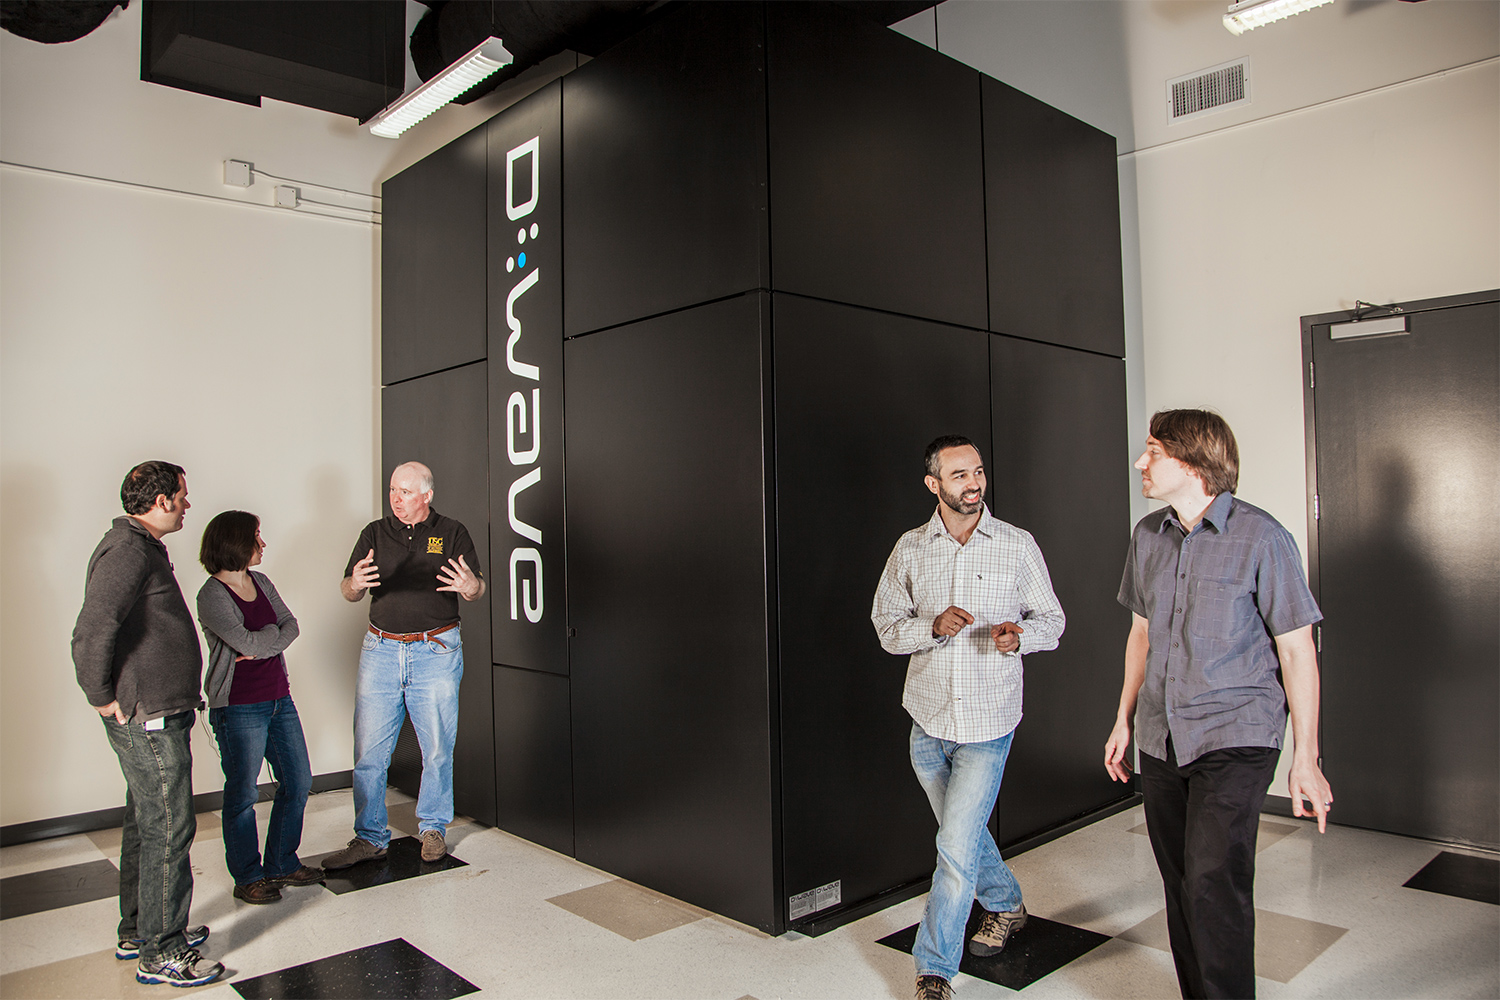
\includegraphics[scale=0.16]{dwave}\footnote{USC Viterbi School of Engineering (Flickr) \url{https://www.flickr.com/photos/uscviterbi/}, via Digital Trends \url{https://www.digitaltrends.com/computing/d-wave-2000-qubit-processor-quantum-computing/}}
\end{center}
\end{frame}

\note{Pictured: People standing in front of a D-Wave quantum computer.}

\begin{frame}
\frametitle{D-Wave 2000Q: The world's largest quantum computer}

\begin{center}
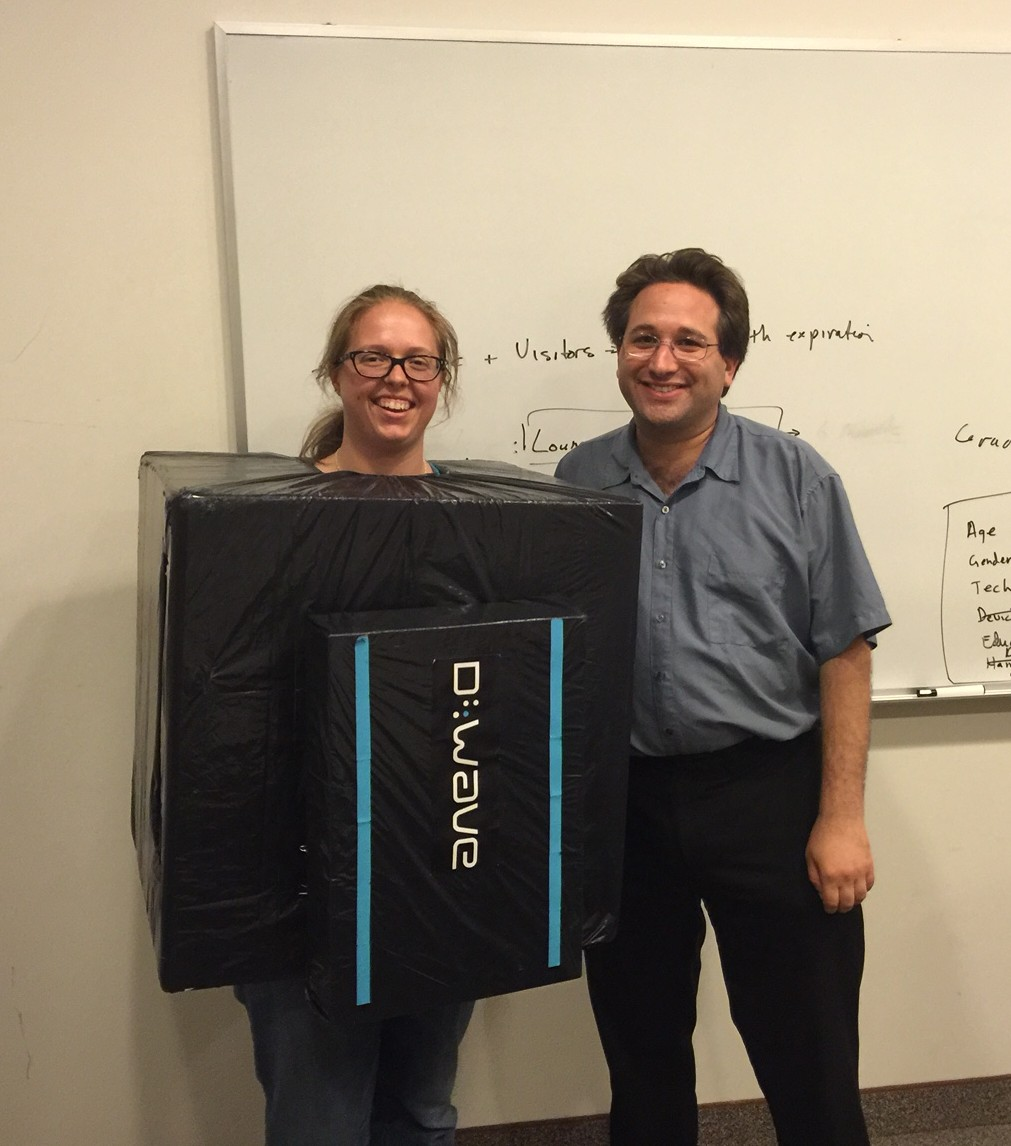
\includegraphics[scale=0.15]{dwavecostume1}
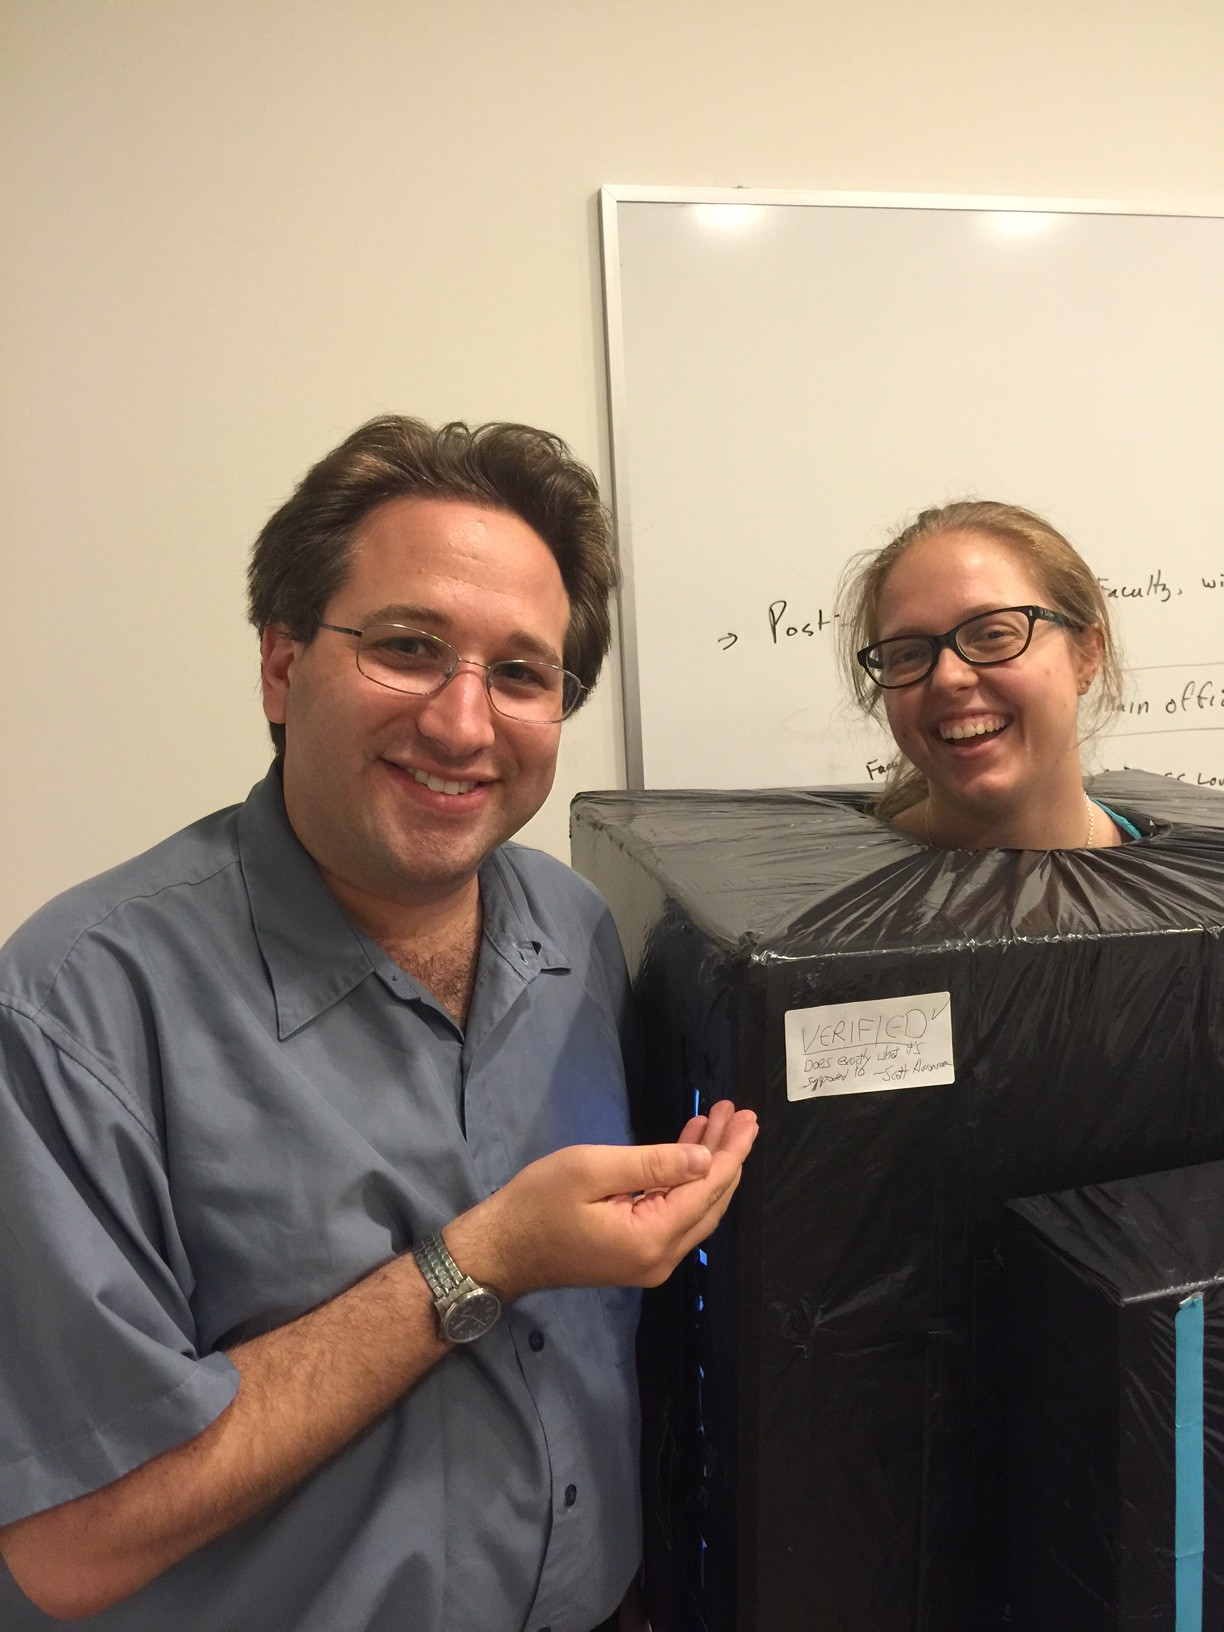
\includegraphics[scale=0.1]{dwavecostume2}\footnote{\url{https://www.scottaaronson.com/blog/?p=2448}}
\end{center}
\end{frame}

\note[itemize]{
\item Pictured left: Sarah Kaiser and Scott Aaronson in front of a whiteboard. Sarah is wearing a costume of a D-Wave quantum computer.
\item Pictured right: Scott Aaronson and Sarah Kaiser. Scott has written on Sarah's costume ``VERIFIED Does exactly what it's supposed to -- Scott Aaronson''.
}

\begin{frame}
\frametitle{How to access a D-Wave machine yourself!}

\begin{itemize}
\item<1-> Buy one, for \$15 million\footnote{\url{https://www.wired.co.uk/article/d-wave-2000q-quantum-computer}}
\item<2-> Rent time on one, cheaper but still pricey
\item<3-> Use Selby's simulator, freely available on GitHub\footnote{\url{https://github.com/alex1770/QUBO-Chimera}}, demonstrated to run faster than earlier D-Wave machines and conjectured to be faster than the 2000Q\footnote{\url{http://www.archduke.org/stuff/d-wave-comment-on-comparison-with-classical-computers/harder-qubo-instances-on-a-chimera-graph/}}
\end{itemize}
\end{frame}

\section{What is a quantum computer?}

\begin{frame}
\frametitle{Warning: Here be \cancel{dragons} mathematics...}

\begin{center}

\includegraphics[scale=0.9]{math}\footnote{Futurama, via Tenor \url{https://tenor.com/view/futurama-math-mathematics-we-need-math-we-need-to-use-math-gif-3486402}}
\end{center}

\end{frame}

\note{Pictured: Bender from TV series Futurama sat in a chair. Caption says ``I'm afraid we need to use...MATH''.}

\begin{frame}
\frametitle{Quantum bits}

Data is represented in a quantum computer as quantum bits (qubits):

$$
|\psi\rangle = \begin{pmatrix}
\alpha\\
\beta
\end{pmatrix} = \alpha|0\rangle + \beta|1\rangle
$$

$$\alpha, \beta \in \mathbb{C}, |\alpha|^2 + |\beta|^2 = 1$$
\end{frame}

\begin{frame}
\frametitle{Quantum gates}

Logical gates in a quantum computer are unitary matrices acting on qubits:

$$
U = \begin{pmatrix}
a & b\\
c & d
\end{pmatrix}
$$

$$U|\psi\rangle = \alpha(a|0\rangle + b|1\rangle) + \beta(c|0\rangle + d|1\rangle)$$
\end{frame}

\begin{frame}
\frametitle{Measurement and output}

When we look at a quantum state $|\psi\rangle$, we find

\begin{itemize}
\item $|0\rangle$ with probability $|\alpha|^2$
\item $|1\rangle$ with probability $|\beta|^2$
\end{itemize}

The state then collapses into the measured result.
\end{frame}

\begin{frame}
\frametitle{A simple quantum simulation algorithm}

Each qubit can be represented as two complex numbers.

A unitary gate operating on a qubit is a $2\times2$ matrix-vector product.

Measurement is just a random number generation.

Doing each of these steps shouldn't take more than $O(n)$.

So where does the complexity come from?
\end{frame}

\section{Interference}

\begin{frame}
\frametitle{Interference}

So far we have assumed the qubits are independent of each other.

$$\frac{|00\rangle + |11\rangle}{\sqrt{2}}$$

Is a valid quantum state.

Measuring each qubit individually gives $|0\rangle$ or $|1\rangle$ with equal probability.

But measuring both qubits together shows that they are perfectly correlated.

\end{frame}

\begin{frame}
\frametitle{Interference makes simulations harder}

We now need to consider the probabilities of qubits collectively.

For $n$ qubits, this means keeping track of $2^n$ complex numbers!
\end{frame}

\begin{frame}
\frametitle{Quantum interference on a D-Wave machine}
\begin{center}
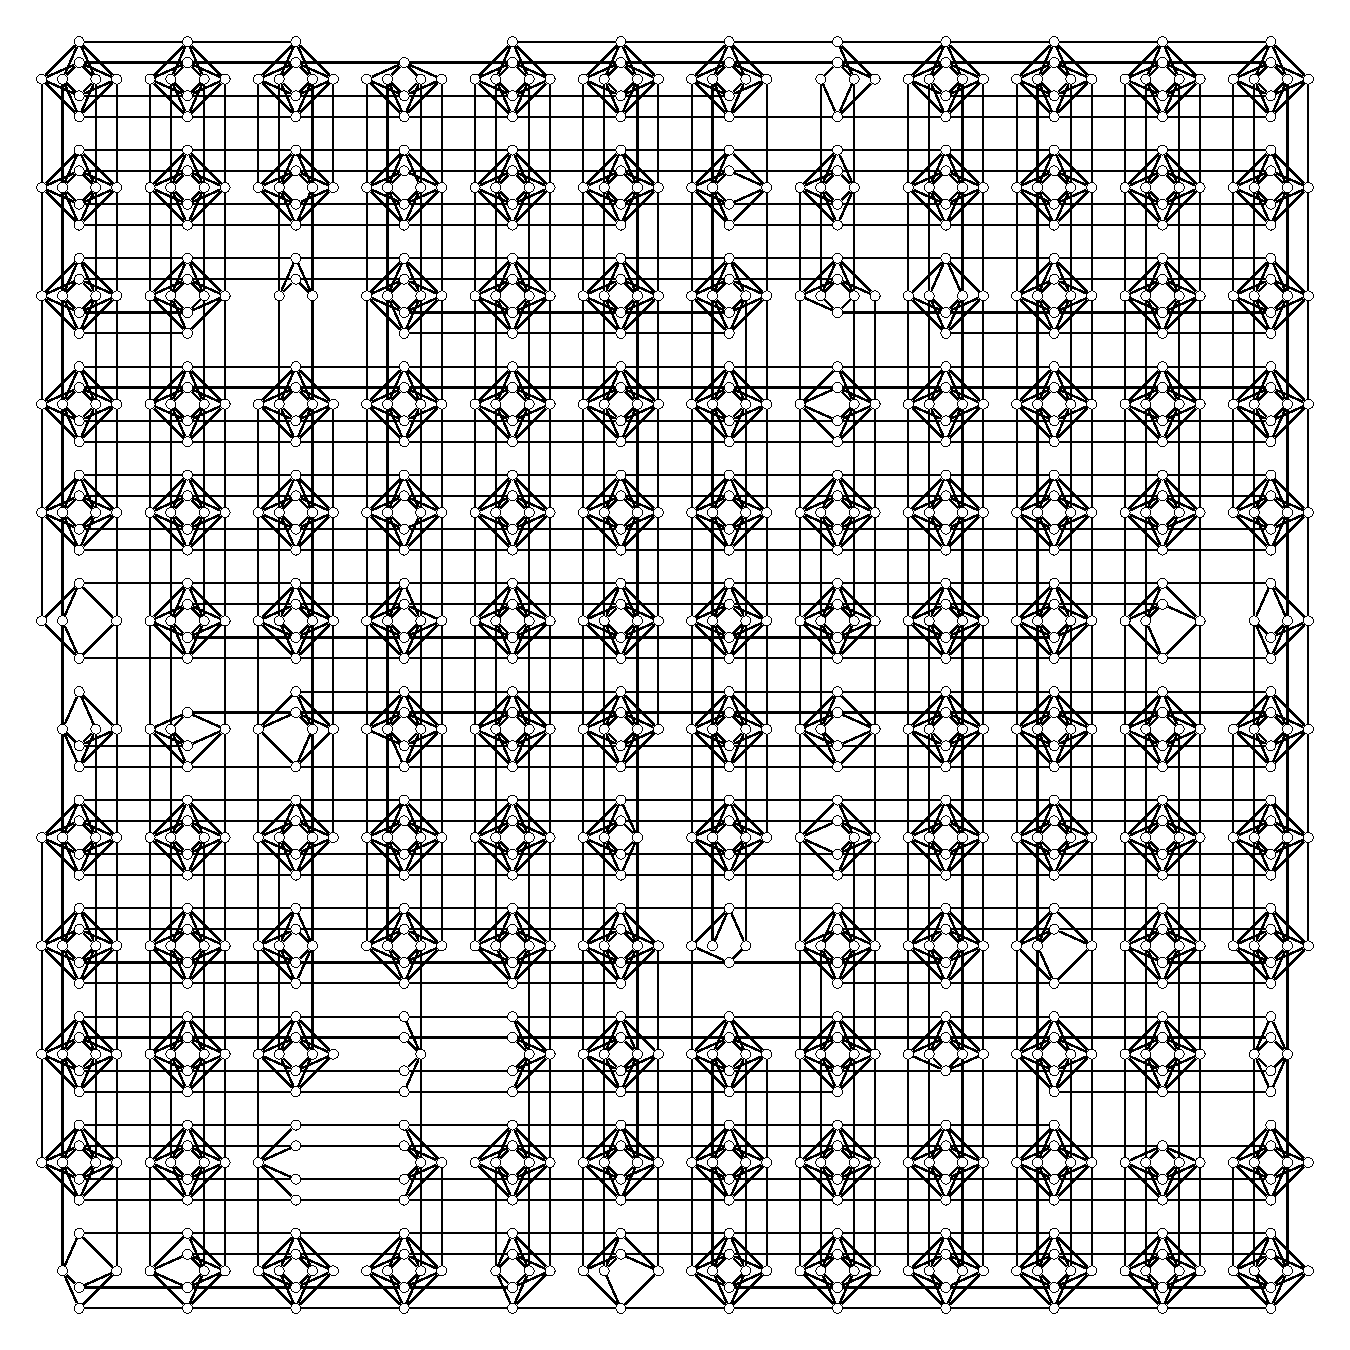
\includegraphics[scale=0.25]{dwave2x}\footnote{King et al., {\tt arXiv:1508.05087}}
\end{center}
\end{frame}

\note{Pictured: Structure of qubits in a D-Wave 2X quantum computer. Circles represent qubits, and two circles connected by a line indicates that those qubits can interact with each other.}

\begin{frame}
\frametitle{Interference on IBM's chips}

IBM have also developed quantum computation chips, which are based on a model which cannot be simulated by Selby's algorithm.

So how many qubits have they got?
\end{frame}

\begin{frame}
\begin{center}
\begin{huge}
16
\end{huge}

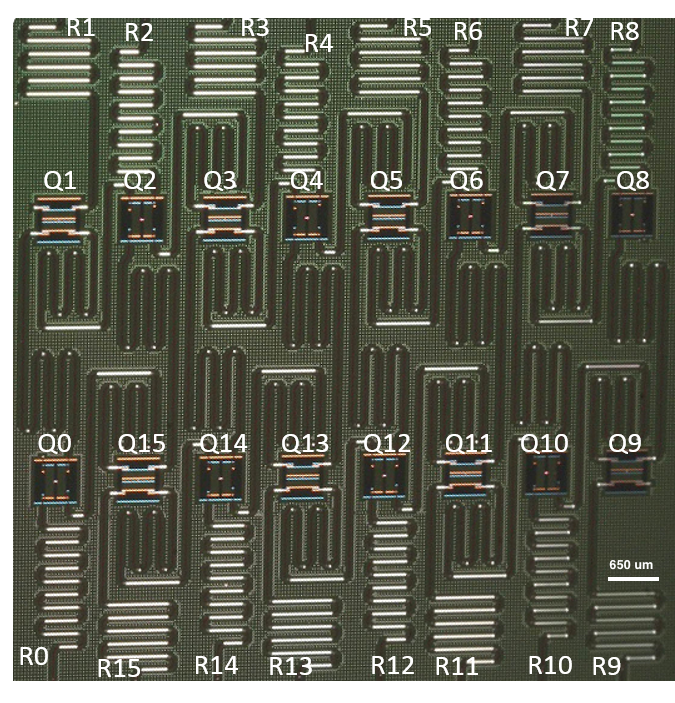
\includegraphics[scale=0.3]{ibmqx3-labeled}\footnote{\url{https://github.com/QISKit/ibmqx-backend-information/blob/master/backends/ibmqx5/README.md}}
\end{center}
\end{frame}

\note{Pictured: IBM QX5 quantum chip. Text overlay indicates each of the qubits, labelled Q0-Q15, and corresponding readout components, labelled R0-R15.}

\section{It's not all doom and gloom}

\begin{frame}
\frametitle{Where do we go from here?}

Getting interaction between every qubit is near impossible.

But significant research is currently going into creating quantum architectures which are hard to simulate and scalable.

The largest device so far is 50 qubits, developed by IBM but not yet public\footnote{\url{https://www-03.ibm.com/press/us/en/pressrelease/53374.wss}}.

There is also significant work on error correction schemes, so that quantum operations can take longer.
\end{frame}

\begin{frame}
\frametitle{Quantum computational advantage}

What is the smallest quantum experiment that is easier to build and run than it is to simulate?

Possible options include\footnote{Harrow \& Montanaro, Nature 549, 203–209 (2017)}
\begin{itemize}
\item Linear optics
\item Random circuits
\item Low depth circuits
\item Nuclear Magnetic Resonance\footnote{Jones, PhysChemComm 11 (2001)}
\end{itemize}
\end{frame}

%------------------------------------------------
\section{Conclusion}
%------------------------------------------------

\begin{frame}
\frametitle{Conclusion}

Quantum computers have a lot of potential to outperform our best classical computers.

But there are lots of hurdles currently in the way.

The need for interaction between qubits is one such hurdle.

Other issues include noise and errors, which build up in quantum states over time.

\end{frame}

%------------------------------------------------
\section{And now a word from our sponsors!}
%------------------------------------------------

\begin{frame}
\frametitle{Quantum Engineering Centre for Doctoral Training}

  \begin{columns}[T]
    \begin{column}{.5\textwidth}
    \begin{center}
    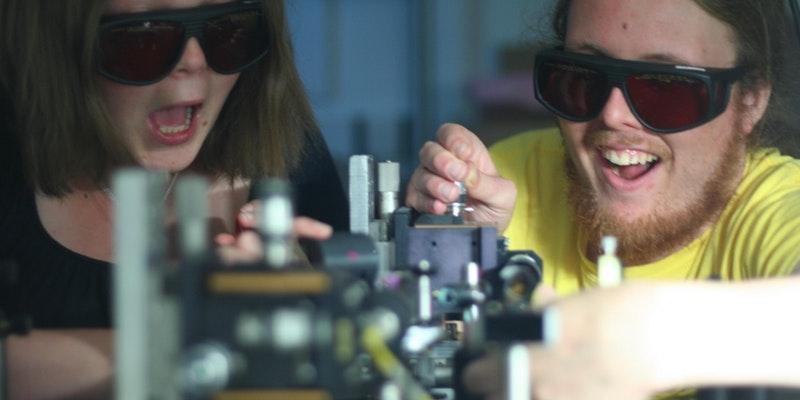
\includegraphics[scale=0.2]{cdt_open_day}
    \end{center}
    \end{column}
    \begin{column}{.5\textwidth}
    \begin{itemize}
    \item 1 year MRes including experimental, theoretical and taught work, plus 3 year PhD on a research project of your choice
    
    \item Fully funded
    
    \item Opportunities to travel and collaborate with other researchers in academia and industry
    \end{itemize}
    \end{column}
  \end{columns}
  
  Open day 5th December: \url{https://www.eventbrite.co.uk/e/quantum-engineering-bristol-tickets-39609797972}

\end{frame}

\note{Pictured: Two PhD students on the Quantum Engineering Centre for Doctoral Training. The students are wearing laser safety goggles and adjusting some optics equipment.}

%------------------------------------------------
\section{The End}
%------------------------------------------------

\begin{frame}
\frametitle{The end}
\begin{center}
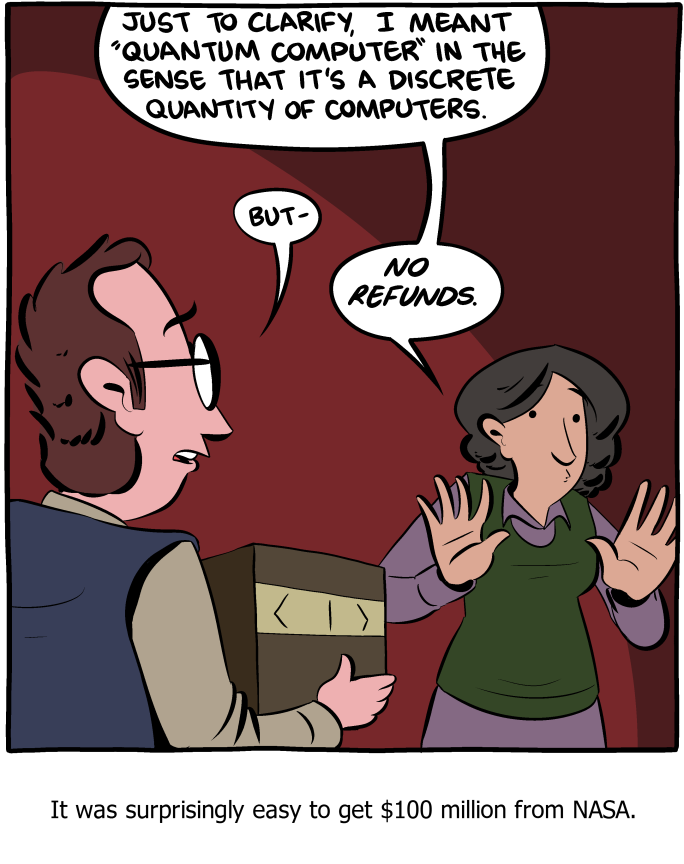
\includegraphics[scale=0.2]{smbc}\footnote{\url{http://www.smbc-comics.com/comic/quantum-computer}}

Any questions?
\end{center}
\end{frame}

\note{Pictured: Comic where a feminine-presenting person on the right has handed a box to a masculine-presenting person on the left. The box has bra-ket notation $\langle|\rangle$ on the side. Dialogue reads:

``Just to clarify, I meant ``quantum computer'' in the sense that it's a discrete quantity of computers.''

``But-''

``No refunds.''

Caption reads: ``It was surprisingly easy to get \$100 million from NASA.''}

%------------------------------------------------
\section{Post-credits}
%------------------------------------------------

\begin{frame}[noframenumbering]
\frametitle{Post-credits}
The slide is as useful as a current-day quantum computer.
\end{frame}

%----------------------------------------------------------------------------------------

\end{document} 
